\documentclass[border=4pt]{standalone}
% Shared TikZ macros for the "Gaussian wave" amplitude diagrams.
% Each wave is drawn isolated inside a fixed-size cell, no axes, with an
% optional probability label placed just outside the bump.
\usepackage{tikz}
\usepackage{amssymb}
\usepackage{amsmath}
\usetikzlibrary{calc,arrows.meta}

\definecolor{waveblue}{HTML}{3A7CA5}
\definecolor{wavered}{HTML}{D1495B}

% \gaussiancell{x0}{y0}{sign}{height}{color}{basislabel}{highlight}{problabel}
% Draws one Gaussian bump centered at (x0,y0), cell width 2.4, height range +-1.1.
% sign: +1 upright, -1 flipped. height: 0..1 (fraction of max bump height 0.85).
% basislabel: basis-state ket, always placed BELOW the baseline; empty string = no label.
% highlight: 1 draws a thin colored box around the cell, 0 = none.
% problabel: probability value, always placed ABOVE the bump's peak; empty string = no label.
\newcommand{\gaussiancell}[8]{%
  \begin{scope}[shift={(#1,#2)}]
    \pgfmathsetmacro{\amp}{#4*0.85*#3}
    \pgfmathsetmacro{\wid}{0.30}
    \draw[black, line width=0.5pt] (-1.15,0) -- (1.15,0);
    \draw[#5, line width=1.3pt, samples=120, smooth, domain=-1.05:1.05]
      plot (\x, {\amp*exp(-(\x*\x)/(2*\wid*\wid))});
    \fill[#5, opacity=0.18, samples=120, domain=-1.05:1.05]
      plot (\x, {\amp*exp(-(\x*\x)/(2*\wid*\wid))}) -- (1.05,0) -- (-1.05,0) -- cycle;
    \ifnum#7=1
      \draw[wavered, line width=0.9pt] (-1.15,-0.65) rectangle (1.15,1.35);
    \fi
    \ifx&#6&
    \else
      \ifnum#3>0
        \node[anchor=north, font=\footnotesize] at (0, -0.35) {#6};
      \else
        \node[anchor=north, font=\footnotesize] at (0, -0.95) {#6};
      \fi
    \fi
    \ifx&#8&
    \else
      \node[anchor=south, font=\small] at (0, 0.95) {#8};
    \fi
  \end{scope}
}

% \wavegrid{rows}{cols}{dx}{dy}{cellfn} where cellfn takes (row,col,index)
% (grid layout handled inline per-figure instead, for full control over per-cell content)

% \meanline{x0}{y0}{width}{amp}{label}
% Draws a dotted horizontal line at height amp (in the same units as
% \gaussiancell's amplitude, i.e. peak height = 0.85 at amp=1) spanning
% `width` cells wide, centered at (x0,y0), with a small label to its right.
\newcommand{\meanline}[5]{%
  \begin{scope}[shift={(#1,#2)}]
    \pgfmathsetmacro{\amp}{#4*0.85}
    \draw[gray, line width=0.9pt, densely dotted] (-1.15,\amp) -- (#3-1.15,\amp);
    \ifx&#5&
    \else
      \node[gray, anchor=west, font=\footnotesize] at (#3-1.05,\amp) {#5};
    \fi
  \end{scope}
}

\begin{document}
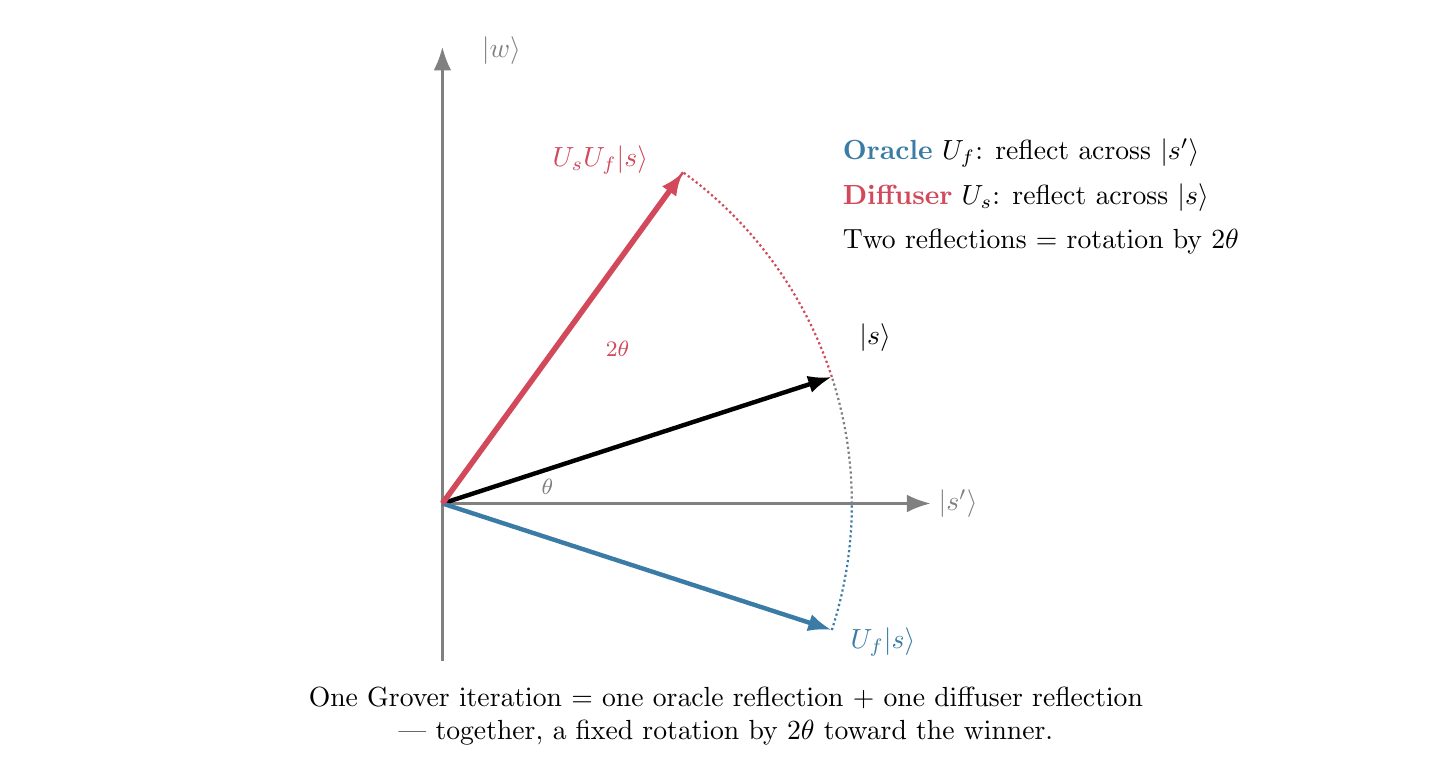
\begin{tikzpicture}
  % Geometry: |s'> along the x-axis, |w> along the y-axis. Start at |s>,
  % angle thetaDeg above |s'>. Oracle reflects across |s'> (the x-axis) to
  % angle -thetaDeg. Diffuser reflects that across |s> (angle thetaDeg) to
  % land at angle 3*thetaDeg -- a net rotation of 2*thetaDeg toward |w>.
  \def\R{5.2}
  \pgfmathsetmacro{\thetaDeg}{18}     % theta, exaggerated for legibility
  \pgfmathsetmacro{\afterOracle}{-\thetaDeg}
  \pgfmathsetmacro{\afterDiffuser}{3*\thetaDeg}

  % ---------- axes ----------
  \draw[-{Latex[length=3mm]}, line width=1pt, gray] (0,0) -- (\R+1.0,0);
  \node[gray, font=\normalsize] at (\R+1.35,0) {$|s'\rangle$};
  \draw[-{Latex[length=3mm]}, line width=1pt, gray] (0,-2.0) -- (0,\R+0.6);
  \node[gray, font=\normalsize] at (0.75,\R+0.55) {$|w\rangle$};

  % ---------- reference: theta wedge from x-axis to |s> ----------
  \draw[gray, densely dotted, line width=0.8pt] (\R,0) arc (0:\thetaDeg:\R);
  \node[gray, font=\footnotesize] at ({1.35*cos(\thetaDeg/2)},{1.35*sin(\thetaDeg/2)}) {$\theta$};

  % ---------- Step 0: |s> ----------
  \draw[black, line width=1.6pt, -{Latex[length=3mm]}] (0,0) -- ({\R*cos(\thetaDeg)},{\R*sin(\thetaDeg)});
  \node[black, font=\normalsize\bfseries] at ({\R*cos(\thetaDeg)+0.55},{\R*sin(\thetaDeg)+0.5}) {$|s\rangle$};

  % ---------- Step 1: after oracle (reflect across |s'>, the x-axis) ----------
  \draw[waveblue, line width=1.6pt, -{Latex[length=3mm]}] (0,0) -- ({\R*cos(\afterOracle)},{\R*sin(\afterOracle)});
  \node[waveblue, font=\normalsize\bfseries] at ({\R*cos(\afterOracle)+0.65},{\R*sin(\afterOracle)-0.15}) {$U_f|s\rangle$};
  \draw[waveblue, densely dotted, line width=0.8pt] ({\R*cos(\afterOracle)},{\R*sin(\afterOracle)}) arc (\afterOracle:0:\R);

  % ---------- Step 2: after diffuser (reflect across |s>) ----------
  \draw[wavered, line width=2pt, -{Latex[length=3mm]}] (0,0) -- ({\R*cos(\afterDiffuser)},{\R*sin(\afterDiffuser)});
  \node[wavered, font=\normalsize\bfseries] at ({\R*cos(\afterDiffuser)-1.05},{\R*sin(\afterDiffuser)+0.15}) {$U_sU_f|s\rangle$};
  \draw[wavered, densely dotted, line width=0.8pt] ({\R*cos(\thetaDeg)},{\R*sin(\thetaDeg)}) arc (\thetaDeg:\afterDiffuser:\R);

  % ---------- 2*theta net-rotation callout ----------
  \draw[wavered, densely dashed, line width=0.9pt] (0,0) -- ({\R*cos(\afterDiffuser)},{\R*sin(\afterDiffuser)});
  \node[wavered, font=\footnotesize] at ({2.75*cos(2*\thetaDeg)},{2.75*sin(2*\thetaDeg)+0.35}) {$2\theta$};

  % ---------- legend ----------
  \node[font=\normalsize, align=left] at (\R+2.4,\R-1.3)
    {\textcolor{waveblue}{\bfseries Oracle} $U_f$: reflect across $|s'\rangle$\\[4pt]
     \textcolor{wavered}{\bfseries Diffuser} $U_s$: reflect across $|s\rangle$\\[4pt]
     Two reflections = rotation by $2\theta$};

  \node[font=\normalsize, text width=17.5cm, align=center] at (\R/2+1,-2.7)
    {One Grover iteration = one oracle reflection + one diffuser reflection\\ --- together, a fixed rotation by $2\theta$ toward the winner.};
\end{tikzpicture}
\end{document}
